%%%%%%%%%%%%%%%%%%%%%%%%%%%%%%%%%%%%%%%%%%%%%%%%%%%%%%%%%%%%%%%%%%%%%%%%%%%%%%%%
%2345678901234567890123456789012345678901234567890123456789012345678901234567890
%        1         2         3         4         5         6         7         8

\documentclass[letterpaper, 10 pt, conference]{ieeeconf}  % Comment this line out
                                                          % if you need a4paper
%\documentclass[a4paper, 10pt, conference]{ieeeconf}      % Use this line for a4
                                                          % paper

\IEEEoverridecommandlockouts                              % This command is only
                                                          % needed if you want to
                                                          % use the \thanks command
\overrideIEEEmargins
% See the \addtolength command later in the file to balance the column lengths
% on the last page of the document

 
% The following packages can be found on http:\\www.ctan.org
%\usepackage{graphics} % for pdf, bitmapped graphics files
%\usepackage{epsfig} % for postscript graphics files
%\usepackage{mathptmx} % assumes new font selection scheme installed
%\usepackage{times} % assumes new font selection scheme installed
%\usepackage{amsmath} % assumes amsmath package installed
%\usepackage{amssymb}  % assumes amsmath package installed
\usepackage[final]{pdfpages}
\usepackage{caption, rotating}
\usepackage{graphics}
\usepackage{array}
\usepackage[export]{adjustbox}
\usepackage[T1]{fontenc}
\usepackage{url}
 
\title{\LARGE \bf
Lowering Depression and Anxiety: A Quantitative Research on the Relationship of Six Common Habits 
on Human's Mental Health
}
 
\author{Dang Quang Hoang, Karthikeyan Marikrishnan \\ Yuqing Ren, Muhammad Hamza Raza, Hadi Sharifi}



\def\@testdef #1#2#3{%
  \def\reserved@a{#3}\expandafter \ifx \csname #1@#2\endcsname
 \reserved@a  \else
\typeout{^^Jlabel #2 changed:^^J%
\meaning\reserved@a^^J%
\expandafter\meaning\csname #1@#2\endcsname^^J}%
\@tempswatrue \fi}

\begin{document}



\maketitle
\thispagestyle{empty}
\pagestyle{empty}


%%%%%%%%%%%%%%%%%%%%%%%%%%%%%%%%%%%%%%%%%%%%%%%%%%%%%%%%%%%%%%%%%%%%%%%%%%%%%%%%
% \begin{abstract}

% This electronic document is a ÒliveÓ template. The various components of your paper [title, text, heads, etc.] are already defined on the style sheet, as illustrated by the portions given in this document.

% \end{abstract}


%%%%%%%%%%%%%%%%%%%%%%%%%%%%%%%%%%%%%%%%%%%%%%%%%%%%%%%%%%%%%%%%%%%%%%%%%%%%%%%%
\section{INTRODUCTION AND PROBLEM STATEMENT}
Depression and anxiety are two widespread types of disorders that cause a tremendous consequence on human life.  
The World Health Organization (WHO) has ranked depression as the fourth leading cause of human disability.
By 2020, it is expected to be the second leading cause \cite{kessler2013epidemiology}. Many researches touch the symptoms of anxiety and depression.
As an example, depression causes health 
complications \cite{verma2017impact}, cardiovascular diseases \cite{bradley2015depression}, in some cases increases 
the risk of cardiovascular diseases by 80\% \cite{penninx2017depression}. In case of anxiety, on average, up to 33.7\% of 
the human populations experience it in their life time \cite{bandelow2015epidemiology}. Anxiety not only affects the human body physically
but also affects learning and reasoning capabilities \cite{spielberger2013effects}\cite{darke1988effects}. 
Undeniably, these are two major risks for human life.
This proposal analyzes data from the Behavioral Risk Factor Surveillance System (BRFSS)\cite{brfss} for several years. 
It tries to find a relationship between six habit factors (physical activity, eating disorder, 
smoking, drinking alcohol, social media, and education/technology) and depression and anxiety. It proposes a
solution that could lead to reduction of depression and anxiety in the society. 

\section{OBJECTIVE}

\noindent\textit{$\circ$ What this research is trying to accomplish?} \newline
\textnormal{
Identifying the relationship between the six factors and depression and anxiety to 
provide guidelines based on the factors in hope to reduce depression and anxiety.
}

\setlength{\parskip}{1em} %give space between paragraph. Except for the first one above.

\par\noindent\textit{$\circ$ How is research in this field is done today; what are the limits of current practice?}\newline
\textnormal{
Majority of research papers on anxiety and depression covers few variables. 
This limits the scope of influence in exacerbating these disorder. 
}

\par\noindent\textit{$\circ$ What's new to this research? Why will it be successful?}\newline
\textnormal{
This research investigates more recent dominant habits. The outcome  of  the  research  provides  
guidance  for  the larger  body of human society. The key to success of this research is the data 
and by using the data we hope to understand depression and anxiety and hopefully find ways to prevent it. 
The type of data we are using is BRFSS which will be analyzed and used in this research.
}

\par\noindent\textit{$\circ$ Who cares?}\newline
\textnormal{
The general public, medical society, insurance industry, and corporation.  Depression  and  anxiety is 
so widespread that it is a part of  human  life  and  it  is  in  interest  of  the society to  
prevent or mitigate  the effect of it.
}

\par\noindent\textit{$\circ$ If this research is successful, what difference and impact will it make, and how do you measure them?}\newline
\textnormal{
We expect to prevent depression and anxiety in our society as much as we can and also mitigate 
the effect it has on people currently. Surveys  such  as  BRFSS  and  local  and  internal 
surveys  can  provide  a  great  measure  on  how  this  research impacted them.
}

\par\noindent\textit{$\circ$ What are the risks and payoffs?}\newline
\textnormal{
The risk is to convince mass public, human resource organizations, and small 
to large companies that the results of this research will indeed assist them 
get better and faster results. The payoffs are happier work, happier life, 
happier families, and happier society.  
}
\par\noindent\textit{$\circ$ How much will it cost?}\newline
\textnormal{
The major cost is the time it will take. The data is available, 
but it needs to be cleaned, information to be extracted and 
analyzed. At this stage, we anticipate 150 to 200 hours of scientific work. 
}

\par\noindent\textit{$\circ$ How long will it take?}\newline
\textnormal{
The research can be done in 3 to 6 months. But we are going to start
with only 6 factors and hopefully start the spark for future research. 
}
\par\noindent\textit{$\circ$ How will progress be measured?}\newline
\textnormal{
The progress of this research is measured by first establishing a clear connection 
between the six habits and anxiety and depression. Second understanding the nature of the cause and effects.
And third by providing the golden 
guidelines for various parties.
}

\setlength{\parskip}{.5em} %stop giving space
\section{LITERATURE REVIEW}

\par\noindent\textit{$\circ$ The effects of physical activity?}\newline
We have studied three research papers.  
The \cite{strohle2009physical} paper provided a survey on the association 
between physical and therapeutic activity on depression and anxiety. 
The \cite{mammen2013physical} paper analyzes multiple databases to identify factors causing depression as 
well as examine whether physical activity prevents depression. Both show that
physical activity reduces and, in some cases, prevents depression and anxiety. 
The criticism on these papers are that they do not pay adequate attention to symptoms 
and approaches to deal with depression and anxiety as well as benefits of exercise training.
Interestingly, the \cite{van2013exploratory} found that there is no 
relation between vigorous physical activity and mental health or well-being. We believe 
the reason of this results is the vigorous nature of physical activity. 

\setlength{\parskip}{1em} %give space again

\par\noindent\textit{$\circ$ The effects of alcohol abuse and smoking?}\newline
We picked four papers \cite{jia2018associations}\cite{strine2008depression}\cite{allan2015effects}\cite{patton1996smoking}
, all corroborated our hypothesis that abusing alcohol and smoking leads to anxiety and depression. Two of the 
researches used the BRFSS data set. These are valuable research to us. Almost all of them did show a shortcoming that 
the effects on mental health goes beyond one to two variables. Interestingly, research \cite{patton1996smoking}  
from 96 advised school to look into using smoke to help teenagers cope with depression. We are not going to use this paper. 
Smoking may temporarily alleviate depression but it leads to more mental and health symptoms. 


\par\noindent\textit{$\circ$ The effects of social media?}\newline
We have studied three research papers in this topic. They show a strong correlation between 
social media and depression and anxiety. The paper \cite{lin2016association} emphasizes on the correlation 
between social media and depression while considering other environmental and factors such as family and financial. 
The second paper \cite{jelenchick2013facebook} analyzes social networking sites and the relation to depression in older 
adolescents. The participants used have small age difference which lowers the risk of many 
environmental factors skewing the results. The third paper \cite{woods2016sleepyteens} analyzes the use of social media 
and how it relates to depression, anxiety, sleep quality and self-esteem in adolescents. 

\par\noindent\textit{$\circ$ The effects of technology/education?}\newline
We have studied three papers \cite{demirci2015relationship}\cite{bjelland2008does}\cite{mezuk2008influence}. All show positive correlation between 
factors such as high usage of smartphone, low education level and type 2 
diabetes, and depression and anxiety. They have confirmed our hypothesis 
that smartphone/education/diabetes are among leading factors of depression 
disorder and anxiety. All three papers touch particular aspects of technology and we think we should follow the same trend.
We may focus on a particular technology, such as cellphone, instead of "technology" in general. 

\par\noindent\textit{$\circ$ The effects of eating disorder?}\newline
The 
first of the three papers \cite{sassaroli2005role} shows that eating disorder leads to stress and anxiety in 
high school girls. The second paper \cite{martz1995relationship} shows that women with eating disorder 
get highly stressed and the stress led to anxiety behaviors. They also concluded that 
traditional female role causes these symptoms. The third paper \cite{striegel2007risk} shows genetically 
some patients are showing symptoms of eating disorder. This genetic issue leads 
to other issues such as depression and anxiety. The criticism we have on these papers that they only pick 
female population. For our research we will use 
these papers nevertheless, we will make sure to use data for both male and female.  

\section{METHODLOGY}
At this point, We are planning to use python/pandas\cite{pandas} to program, openRefine\cite{openrefine} to clean data, and D3\cite{d3} for visualization.
This may change when the project evolves. 
Each member will extract data from topic assigned to them, clean it, and format it. From that point, we analyze the data, get conclusions, and produce the guidelines.  
Figure \ref{fig:schedule} shows the details on how various tasks are distributed among team members 
and how the timeline is formed to reach all the deadlines. 

%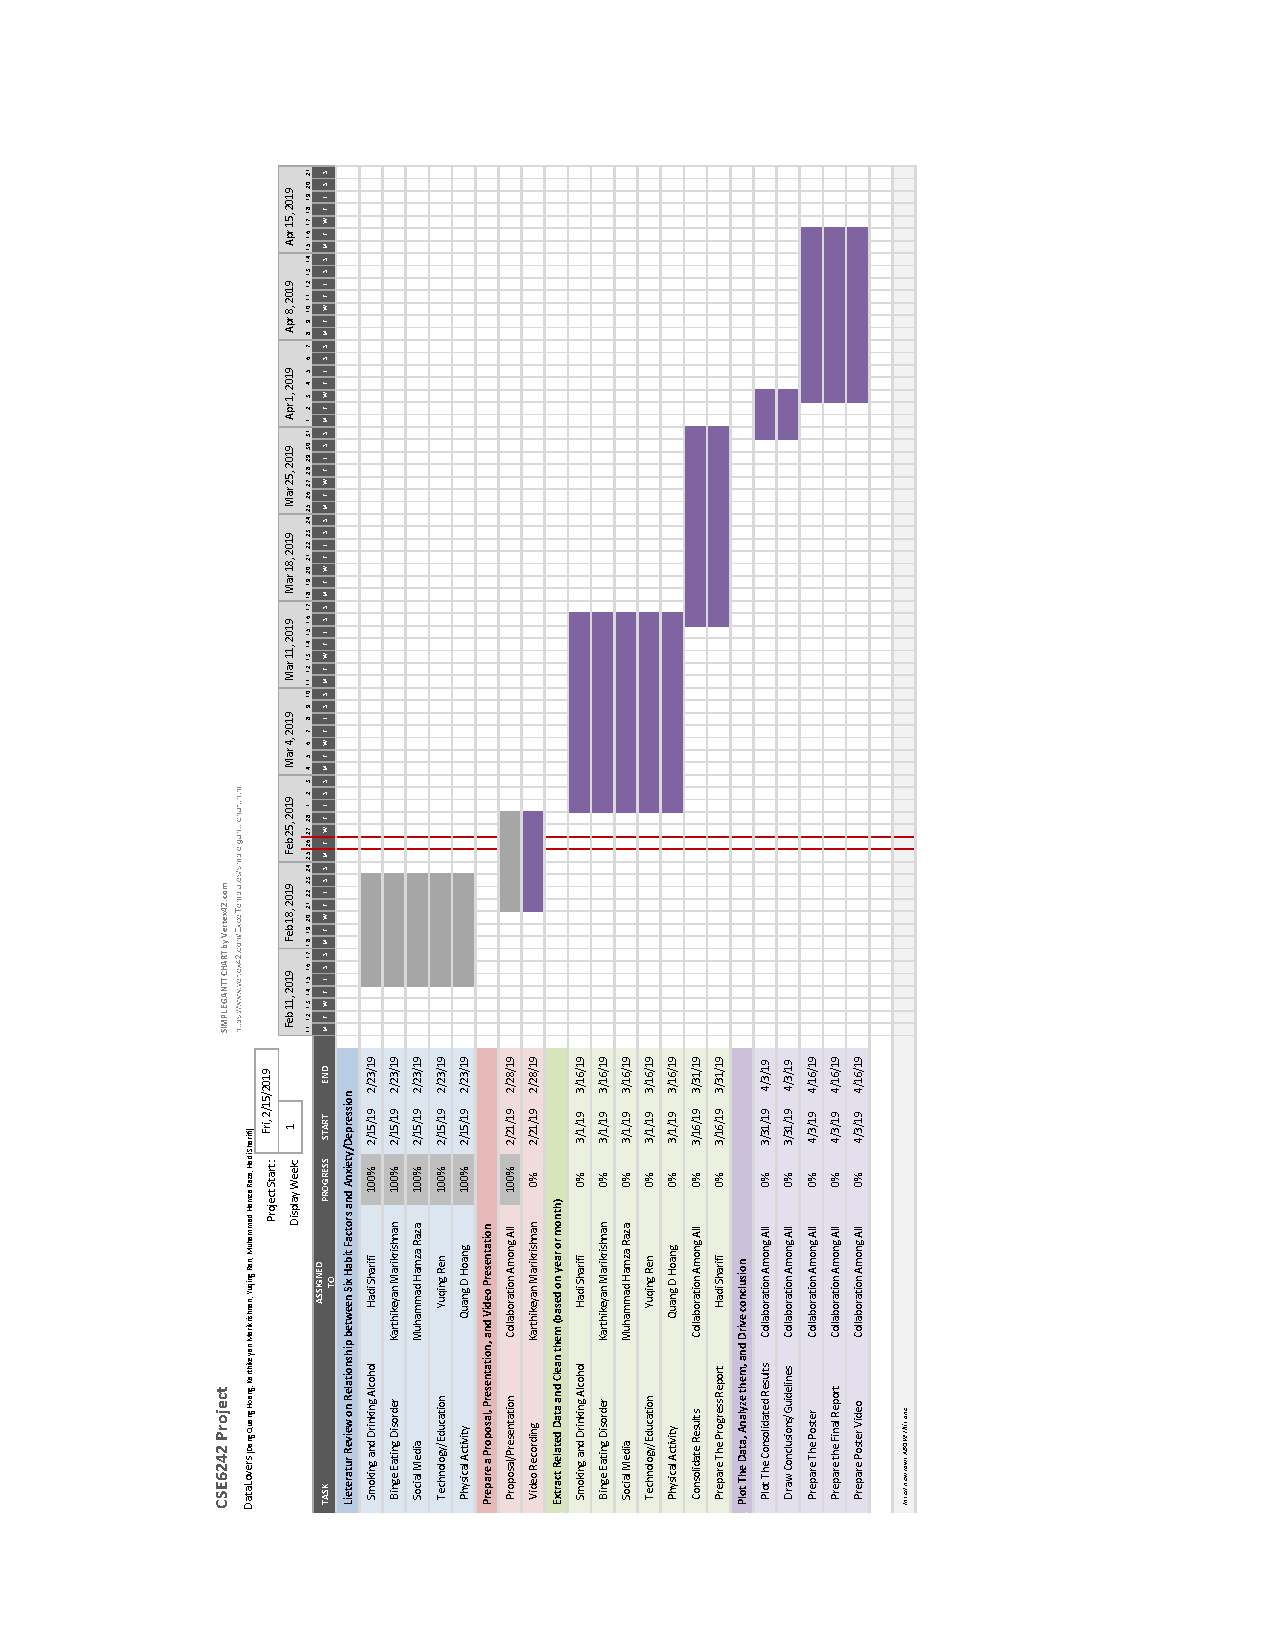
\includepdf{schedule.pdf}
\captionsetup[figure]{labelformat=empty}
\clearpage 
\begin{figure}[hbt!]
        \centering
        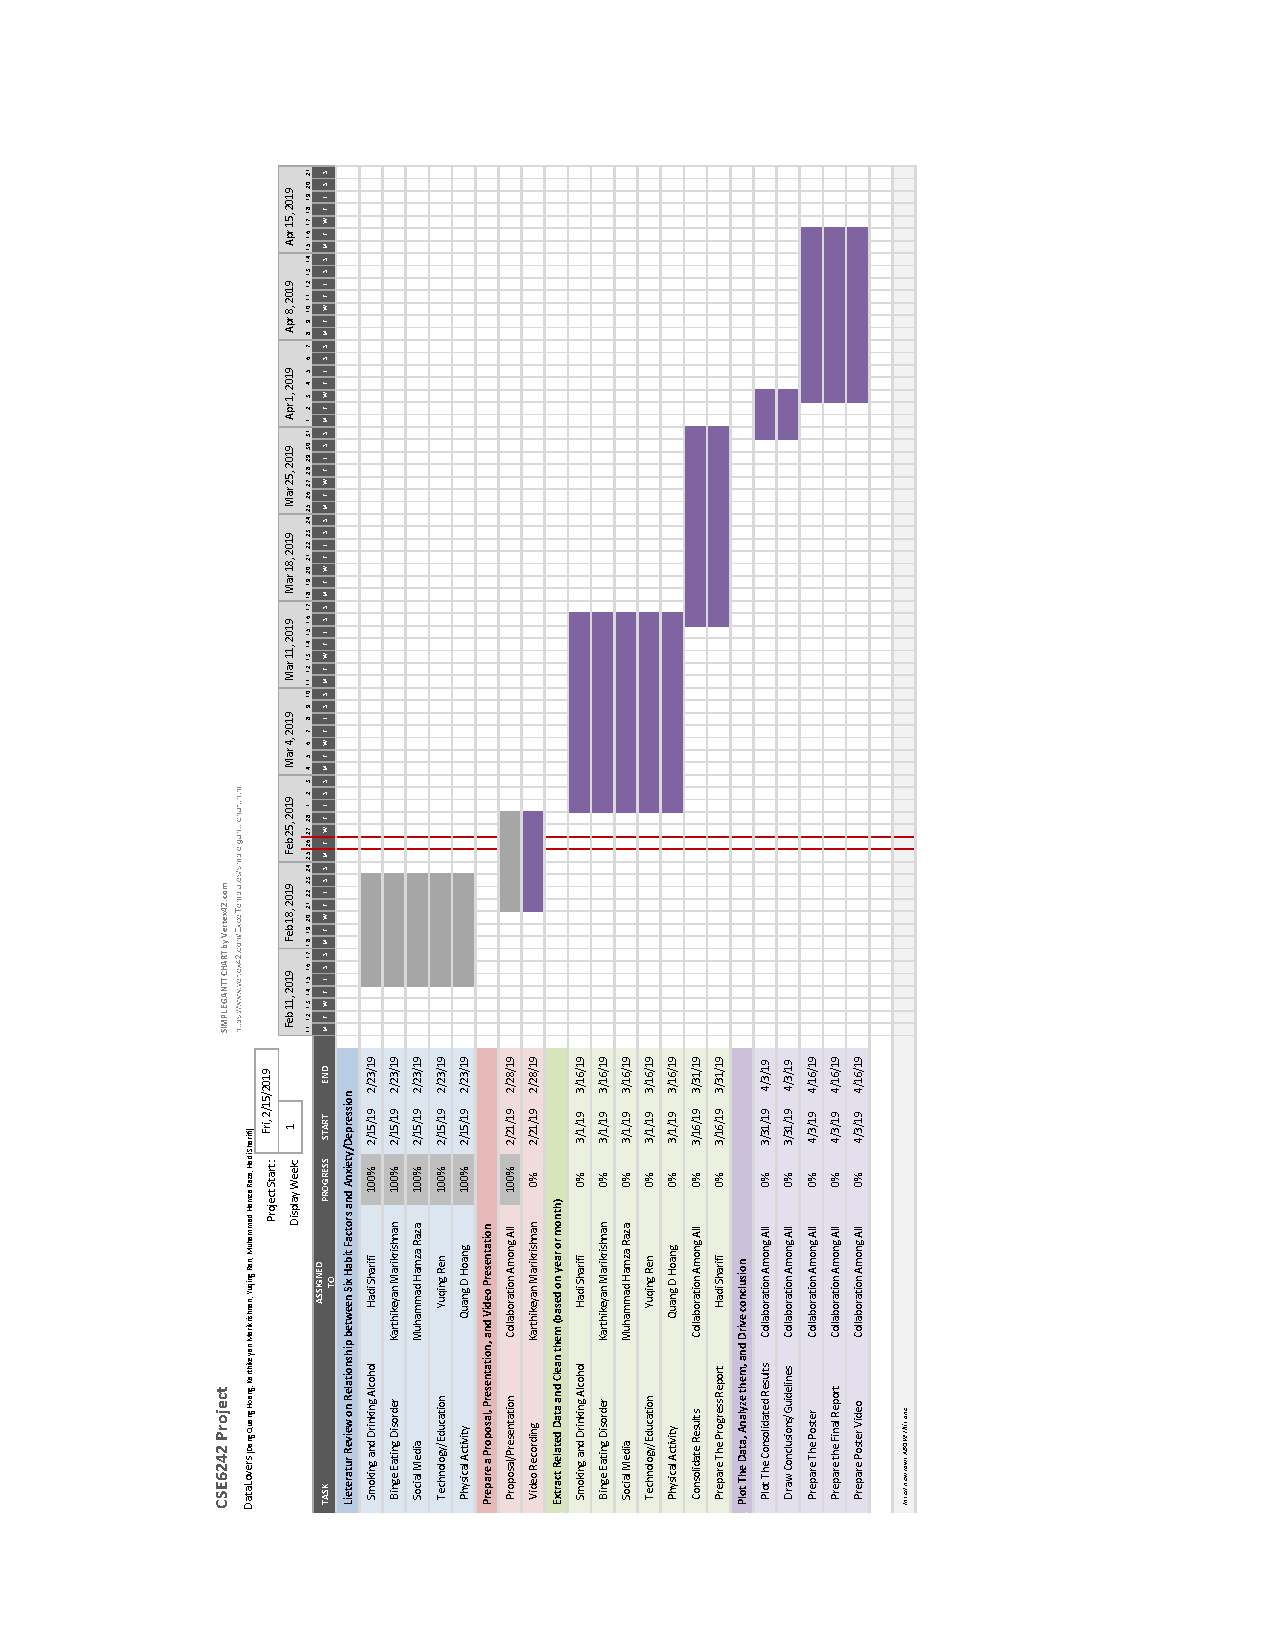
\includepdf[pages=-]{schedule.pdf}
        \addvspace{250pt}
        
        \hspace{-10cm}
        \rotatebox{90}{ Figure ~\ref{fig:schedule}: The schedule of the team for the research.}
        
        %\caption{The Schedule of all tasks defined for the team.}
        \caption{}
        \label{fig:schedule}
\end{figure}

\clearpage 


\bibliography{biblio}
\bibliographystyle{plain}

\section{Appendix}
\begin{figure}[!htb]
        \center{\includegraphics[width=\linewidth]
        {wordcount.png}}
        \caption{\label{fig:my-label} The total number of words in the proposal.}
\end{figure}

\end{document}
